\chapter{Esettanulmány}

Az esettanulmányomnak a célja, hogy egy példán keresztül bemutassam az általam fejlesztett elemző eszköz valamint a rendszermodellből való származtatásnak a folyamatát.

Az esettanulmányom tárgyaként az elektronikus vezérlő egységek (ECU) diagnosztikai szolgáltatását választottam. Ennek oka egyrészről az, hogy az elemzett diagnosztikai szolgáltatások specifikációja publikusan elérhető az ISO 14229 "Road vehicles - Unified Diagnostic Services (UDS)" \cite{ISO14229} szabványban. Másrészről ez egy olyan potenciális belépőpontja lehet a támadóknak amely nem igényel semmiféle fizikai hozzáférést a járműhöz. Amennyiben távolról sikeresen hozzáfér és átveszi az irányítását a támadó egy elektronikus vezérlő egységnek, ami képes V2X vagy más vezetéknélküli szolgáltatásra, onnantól kezdve a jármű többi részén lévő diagnosztikai szolgáltatások is elérhetővé válhatnak számára.\\

Az ISO 14229\cite{ISO14229} definiálja az Unified Diagnostic Services (röviden UDS) protokollt ami egy alkalmazásrétegbeli szolgáltatás. Általános IT biztonsági szempontból, ehhez legközelebbinek a TLS és HTTPS protokollok lennének mondhatók.

\begin{figure}[!ht]
	\centering
	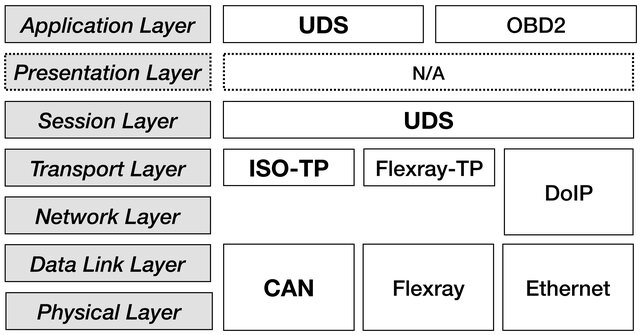
\includegraphics[width=120mm, keepaspectratio]{figures/06_isoosi.jpg}
	\caption{ISO/OSI modell autóipari kommunikációs protokollokra\cite{ISOOSI}}
\end{figure}

Az esettanulmányomban a szolgáltatások közül kettővel, a diagnosztikai autentikációval, valamint a software frissítéssel fogok foglalkozni, mivel ezek a kiemelten kiberbiztonsági relevanciával rendelkező szolgáltatások.\\

A diagnosztikai autentikációt két módon lehet implementálni. Az egyik a \textbf{Security Access (0x27)} a másik pedig a korszerűbb \textbf{Authentication (0x29)} lenne. 

A \textbf{Security Access}-szel az úgynevezett challange-response autentikációt lehet megvalósítani, amelynek a menete először egy valamilyen ismeretlen ECU-n belüli információnak (\textit{seed}) a szolgáltatása a diagnosztikai tesztelő részére, aki ezt az információt valamilyen közös titok (pl: szimmetrikus kulcs) használatával előállít egy kulcsot, amelyet elküld az ECU-nak. Az ECU a fogadó oldalon ellenőrzi, hogy a kulcs ami érkezett az megegyezik azzal amit ugyanezen közös titok és algoritmus használatával állított elő a \textit{seed} lekérése után. Amennyiben a kulcsok megegyeznek az ECU a felhasználót átengedi magasabb biztonsági szinthez ezzel hozzáférést biztosítva korábban nem elérhető diagnosztikai szolgáltatásokhoz.

Az \textbf{Authentication} már egy jóval komplexebb, tanúsítvány alapú autentikációt tesz lehetővé. Ennek a bemutatása túl mutat a jelen esettanulmányon.\\

A szoftverfrissítés egy több lépésből álló szekvenciája diagnosztikai rutin hívásoknak, amelyeket a szabvány "Upload download functional unit" fejezetében fejt ki.

Annak a folyamata, hogy egy új szoftver kerüljön fel az ECU-ra jellemzően a következő lépésekből áll:
\begin{itemize}
	\item \textbf{RequestDownload (0x34)}: Előfeltételek ellenőrzése, letöltési kérelem jóváhagyása
	\item \textbf{TransferData (0x36)}: Adatok feltöltése
	\item \textbf{RequestTransferExit (0x37)}: Érkezett adatok ellenőrzése, jóváhagyás, szoftver indíthatóvá tétele
\end{itemize}

Ezt a folyamat természetesen bővíthető további vagy ezeket megelőző lépésekkel, illetve az egyes rutinok belső működése sincs szabályozva. Maga a kerete viszont egy szoftverfrissítésnek az jellemzően ilyen diagnosztikai szolgáltatások futtatásával és kérések kiszolgálásával történnek az elektronikus vezérlőegységeken.

Érdemes kiemelni itt, hogy ez a frissítési metódus eleinte a járműszervizben történt volna a szerelő által, de a napjainkban már ezeknek a távoli elérése, jellemzően egy külön erre integrált elektronikus vezérlőegység által is lehet lefolytatva. Ezeknek sokban kényelmi, de szintén szoftveres sérülékenységek vagy hibák javítása szempontjából is fontos szerepük van.\\

A protokoll egyébként tartalmaz olyan szolgáltatásokat mint a \textbf{Routine Control (0x31)} amellyel a beszállító és a vevő az eszközre specifikus, nem szabványos diagnosztikai szolgáltatásokat is definiálhat. Ilyenek lehetnek kulcs és tanúsítványkezelő rutinok.

\section{Károkozások és értékek azonosítása}

A \ref{fig:diag_abuse} ábrán láthatóak a potenciális károkozások. A korábban meghatároztuk a két fő szolgáltatást ami az esettanulmányban elemzésre kerül, majd ezekhez a CIA triád mentén való elemzés szerint meghatározásra kerültek a potenciális károkozások. Továbbá egy egy azonosító is került a károkozások nevébe, valamint a felvett sztereotípiával az attributálást is el lehetett végezni.

\begin{itemize}
	\item \textbf{DS-SECDIAG-00 Leak confidential data}: Amennyiben az autentikációs szolgáltatás bizalmassága elveszik, abban az esetben a támadónak lehetősége lesz a bizalmas diagnosztikai adatok kiolvasására
	\item \textbf{DS-SECDIAG-01 Acces unauthorized functionality}: Az autentikációs szolgáltatás integritásának a megtörése vezethet olyan szolgáltatások elérhetővé válásához amelyek normális esetben nem lennének elérhetőek
	\item \textbf{DS-SECDIAG-02 Block authentication attempts}: Az autentikációs szolgáltatás elérhetőségének a blokkolásával korlátozható jogosult felhasználóknak a korlátozott szolgáltatásokhoz való hozzáférése
	\item \textbf{DS-SECSW-00 Leak software}: A szoftver kiszivárogtatásával lehetőség adódik a szoftverben sérülékenységek keresésére, annak kihasználását könnyebbé téve
	\item \textbf{DS-SECSW-01 Change software}: A szoftver megváltoztatásával kártékony szoftver is feljuttatható az elektronikus vezérlőegységre
	\item \textbf{DS-SECSW-02 Remove software}: A szoftver elérhetőségének korlátozásával az elektronikus vezérlőegység teljes funkcionalitása blokkolhatóvá tehető
\end{itemize}

\begin{figure}[!ht]
	\centering
	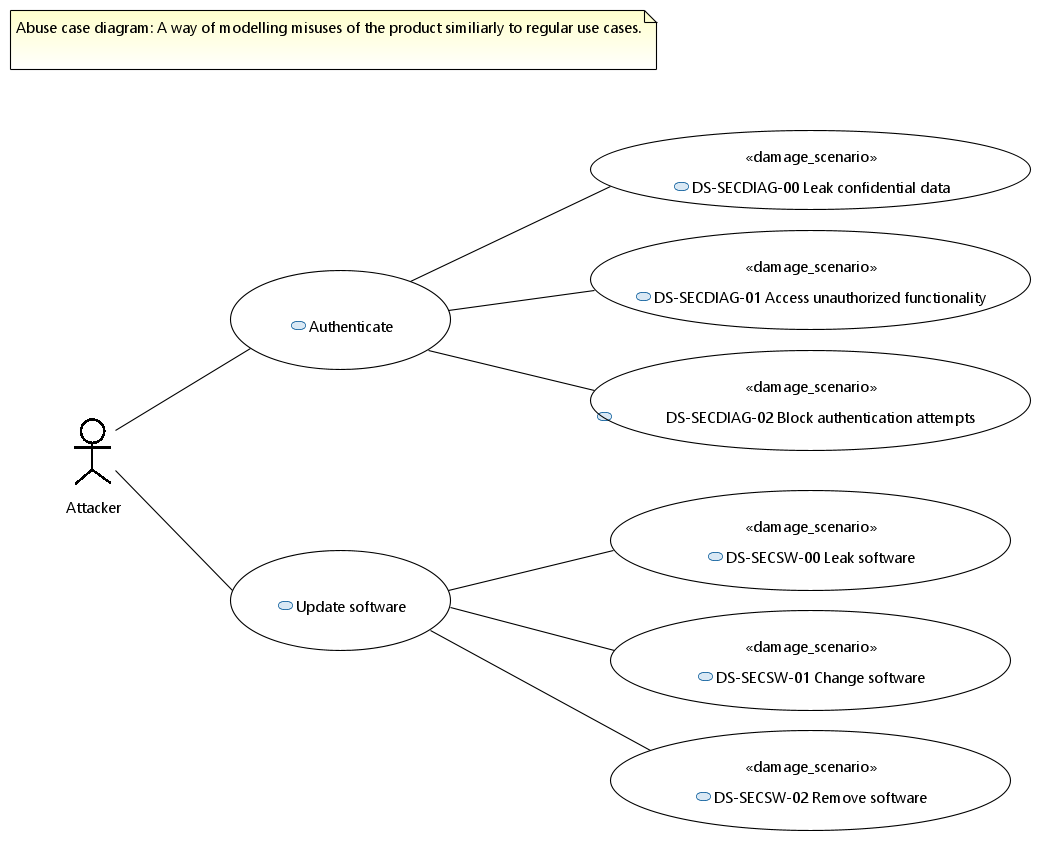
\includegraphics[width=120mm, keepaspectratio]{figures/06_01_abuse_case_diagram.PNG}
	\caption{Diagnosztika kihasználási esetei}
	\label{fig:diag_abuse}
\end{figure}

A termékleíráshoz funkcionalitásokat definiáltuk, kellenek még az ezek által dependált értékek. HW-es komponensből egyedül a CAN csatlakozó hozható fel hiszen azon fog keresztül utazni a bejövő UDS üzenet. SW-szintű értékekből vehetjük a CAN üzenetet amiben utazik az UDS üzenet, maga az UDS üzenet, valamint az az által szállított adatok. Ez a szállított adat a szoftverfrissítés esetén a szoftver lesz, egyébként pedig diagnosztikai adatok lehetnek elérhetőek kiolvasásra az autentikációt követően.

A termékleírás ábrázolva a \ref{fig:item_def} ábrán látható. A sztereotípiák felvétele után volt lehetőségem az attributálásra, ezt a következőképpen tettem meg:
\begin{itemize}
	\item \textbf{Diagnostic Authentication}: A károkozásokból származtathatóan a CIA minden tulajdonsága vonatkozik a funkcionalitásra
	\item \textbf{Software Update}: A károkozásokból származtathatóan a CIA minden tulajdonsága vonatkozik a funkcionalitásra
	\item \textbf{CAN Connector}
	\subitem Sértetlenség: Egy CAN csatlakozó integritását megsértve, kártékony eszközökkel kerülhet kapcsolatba az elemzés tárgyaként szereplő ECU
	\subitem Elérhetőség: Egy CAN csatlakozó elérhetőségét megsértve, a beérkező üzenetek hiányára kell felkészülni
	\item \textbf{CAN Message}
	\subitem Bizalmasság: Az üzenet tartalmazhat bizalmas információt amely segíthet további támadások esetén
	\subitem Sértetlenség: Az üzenet tartalma változtatható, ezzel a fogadó félnél kiváltott reakció is
	\subitem Elérhetőség: Az üzenet blokkolható, a hiánya a fogadó félnél nem zárható ki
	\item \textbf{UDS Message}
	\subitem Bizalmasság: Az üzenet tartalmazhat bizalmas információt amely segíthet további támadások esetén
	\subitem Sértetlenség: Az üzenet tartalma változtatható, ezzel a fogadó félnél kiváltott reakció is
	\subitem Elérhetőség: Az üzenet blokkolható, a hiánya a fogadó félnél nem zárható ki
	\item \textbf{Software}
	\subitem Bizalmasság: A szoftver a fejlesztő cég szellemi tulajdona, ennek kiszivárgása egyrészről anyagi kárt, másrészről további támadások elvégzését is segítheti
	\subitem Sértetlenség: A szoftver változtatható, ezzel a futtató ECU működése is
	\subitem Elérhetőség: A szoftver törölhető, hiánya az ECU biztonságos működését befolyásolhatja
	\item \textbf{Diagnostic Data}
	\subitem Bizalmasság: Az üzenet tartalmazhat bizalmas információt amely segíthet további támadások esetén
\end{itemize}

\begin{figure}[!ht]
	\centering
	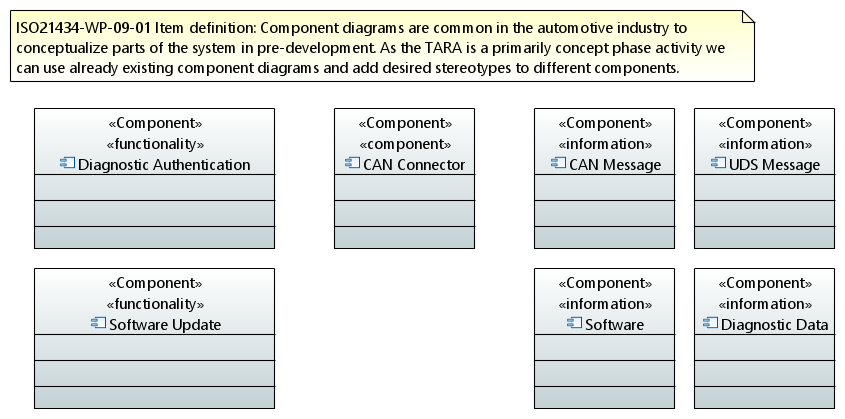
\includegraphics[width=120mm, keepaspectratio]{figures/06_02_item_definition_diagram.PNG}
	\caption{Diagnosztika termékleírása}
	\label{fig:item_def}
\end{figure}

\section{Fenyegetésmodell származtatása}

Az Acceleo szkript futtatása a következő fájlt hozza létre Diagnostics.apeditor néven:

\begin{lstlisting}[basicstyle=\tiny]
<apeditor:ThreatModel xmi:version="2.0" xmlns:xmi="http://www.omg.org/XMI" xmlns:xsi="http://www.w3.org/2001/XMLSchema-instance" xmlns:apeditor="hu.bme.mit.thesis.apeditor">
<damagescenarios name="DS-SECSW-00 Leak software" lossOfConfidentiality="true" lossOfIntegrity="false" lossOfAvailability="false"/>
<damagescenarios name="DS-SECSW-01 Change software" lossOfConfidentiality="false" lossOfIntegrity="true" lossOfAvailability="false"/>
<damagescenarios name="DS-SECSW-02 Remove software" lossOfConfidentiality="false" lossOfIntegrity="false" lossOfAvailability="true"/>
<damagescenarios name="DS-SECDIAG-00 Leak confidential data" lossOfConfidentiality="true" lossOfIntegrity="false" lossOfAvailability="false"/>
<damagescenarios name="DS-SECDIAG-01 Access unauthorized functionality" lossOfConfidentiality="false" lossOfIntegrity="true" lossOfAvailability="false"/>
<damagescenarios name="DS-SECDIAG-02 Block authentication attempts" lossOfConfidentiality="false" lossOfIntegrity="false" lossOfAvailability="true"/>
<asset xsi:type="apeditor:Functionality" name="Software Update"/>
<asset xsi:type="apeditor:Functionality" name="Diagnostic Authentication"/>
<asset xsi:type="apeditor:Component" name="CAN Connector" confidentiality="false" integrity="true" availability="true"/>
<asset xsi:type="apeditor:Information" name="CAN Message" confidentiality="true" integrity="true" availability="true"/>
<asset xsi:type="apeditor:Information" name="UDS Message" confidentiality="true" integrity="true" availability="true"/>
<asset xsi:type="apeditor:Information" name="Software" confidentiality="true" integrity="true" availability="true"/>
<asset xsi:type="apeditor:Information" name="Diagnostic Data" confidentiality="true" integrity="false" availability="false"/>
</apeditor:ThreatModel>
\end{lstlisting}

\section{Fenyegetésmodellezés}

A generált fájl innentől beimportálható és megnyitható olyan Eclipse környezettel amelyhez az elemzőeszköz plugin fájljai hozzá vannak adva.

A dependenciák meghatározásánál a károkozásokhoz hozzátudjuk rendelni a funkcionalitást viszonylag egyértelműen, maga az azonosítójuk is jelzi melyik károkozás melyik funkcióhoz tartozik.

Továbbá mindkét funkcionalitáshoz tartozik a \textbf{CAN Connector} mint HW komponens valamint a \textbf{CAN Message} és \textbf{UDS Message} mint információ. Amiben a két funkcionalitás eltér, hogy ameddig a \textbf{Software Update} esetén az érkező üzenetek a \textbf{Software}-t tartalmazzák, addig az autentikáció után elsősorban a kimenő \textbf{Diagnostic Data} az érték amit védeni akarunk.

Ebből generált majd megszerkesztett hibafák és elemzésük alább megtekinthető. \\
\newpage

\section{Támadási fa analízis}

Ahogy az a \ref{fig:ff_leak_sw} ábrán látható a gyökér fenyegetés a \textbf{Software Update} bizalmasságának sértését okozó \textit{Disclosure of Software Update} lesz. Ez azt jelenti, hogy ezt a funkcionalitást vagy az ehhez tartozó diagnosztikai rutinokat olyan módon használják amellyel bizalmas információkhoz juthat a támadó.

Először levontam a következtetést, hogy egyrészről minden lehetséges támadás azzal fog kezdődni, hogy a támadó valahogyan sérti az integritását a CAN busznak vagy a rendszer csatlakozóján vagy az ahhoz kapcsolódó elemek módosításával. Ez jelenthet fizikai hozzáférést vagy amennyiben egy csatlakoztatott eszköz felett szerez irányítást a támadó, abban az esetben ez akár távolról is elvégezhető.

Másodsorban két támadási irányt különítettem el, az egyik esetben a támadó megpróbál olyan diagnosztikai szolgáltatásokat használni amelyekkel a telepített szoftver kinyerhető lenne az eszközből. A másik esetben az éppen folyamatban lévő szoftverfrissítésnél érkező üzenetek lehallgatásával és azok tartalmának visszafejtésével próbálhat a támadó a szoftverhez hozzájutni. Előbbi esetben egy CAN üzenet lehallgatásával (disclosure) hozzájut a CAN ID-khoz és paraméterekkel, majd módosított üzeneteket injektál amelyekkel a szoftver letöltését kezdeményezheti. A másik esetben UDS üzenet lehallgatás és a szoftver visszafejtése történne.

\begin{figure}[!ht]
	\centering
	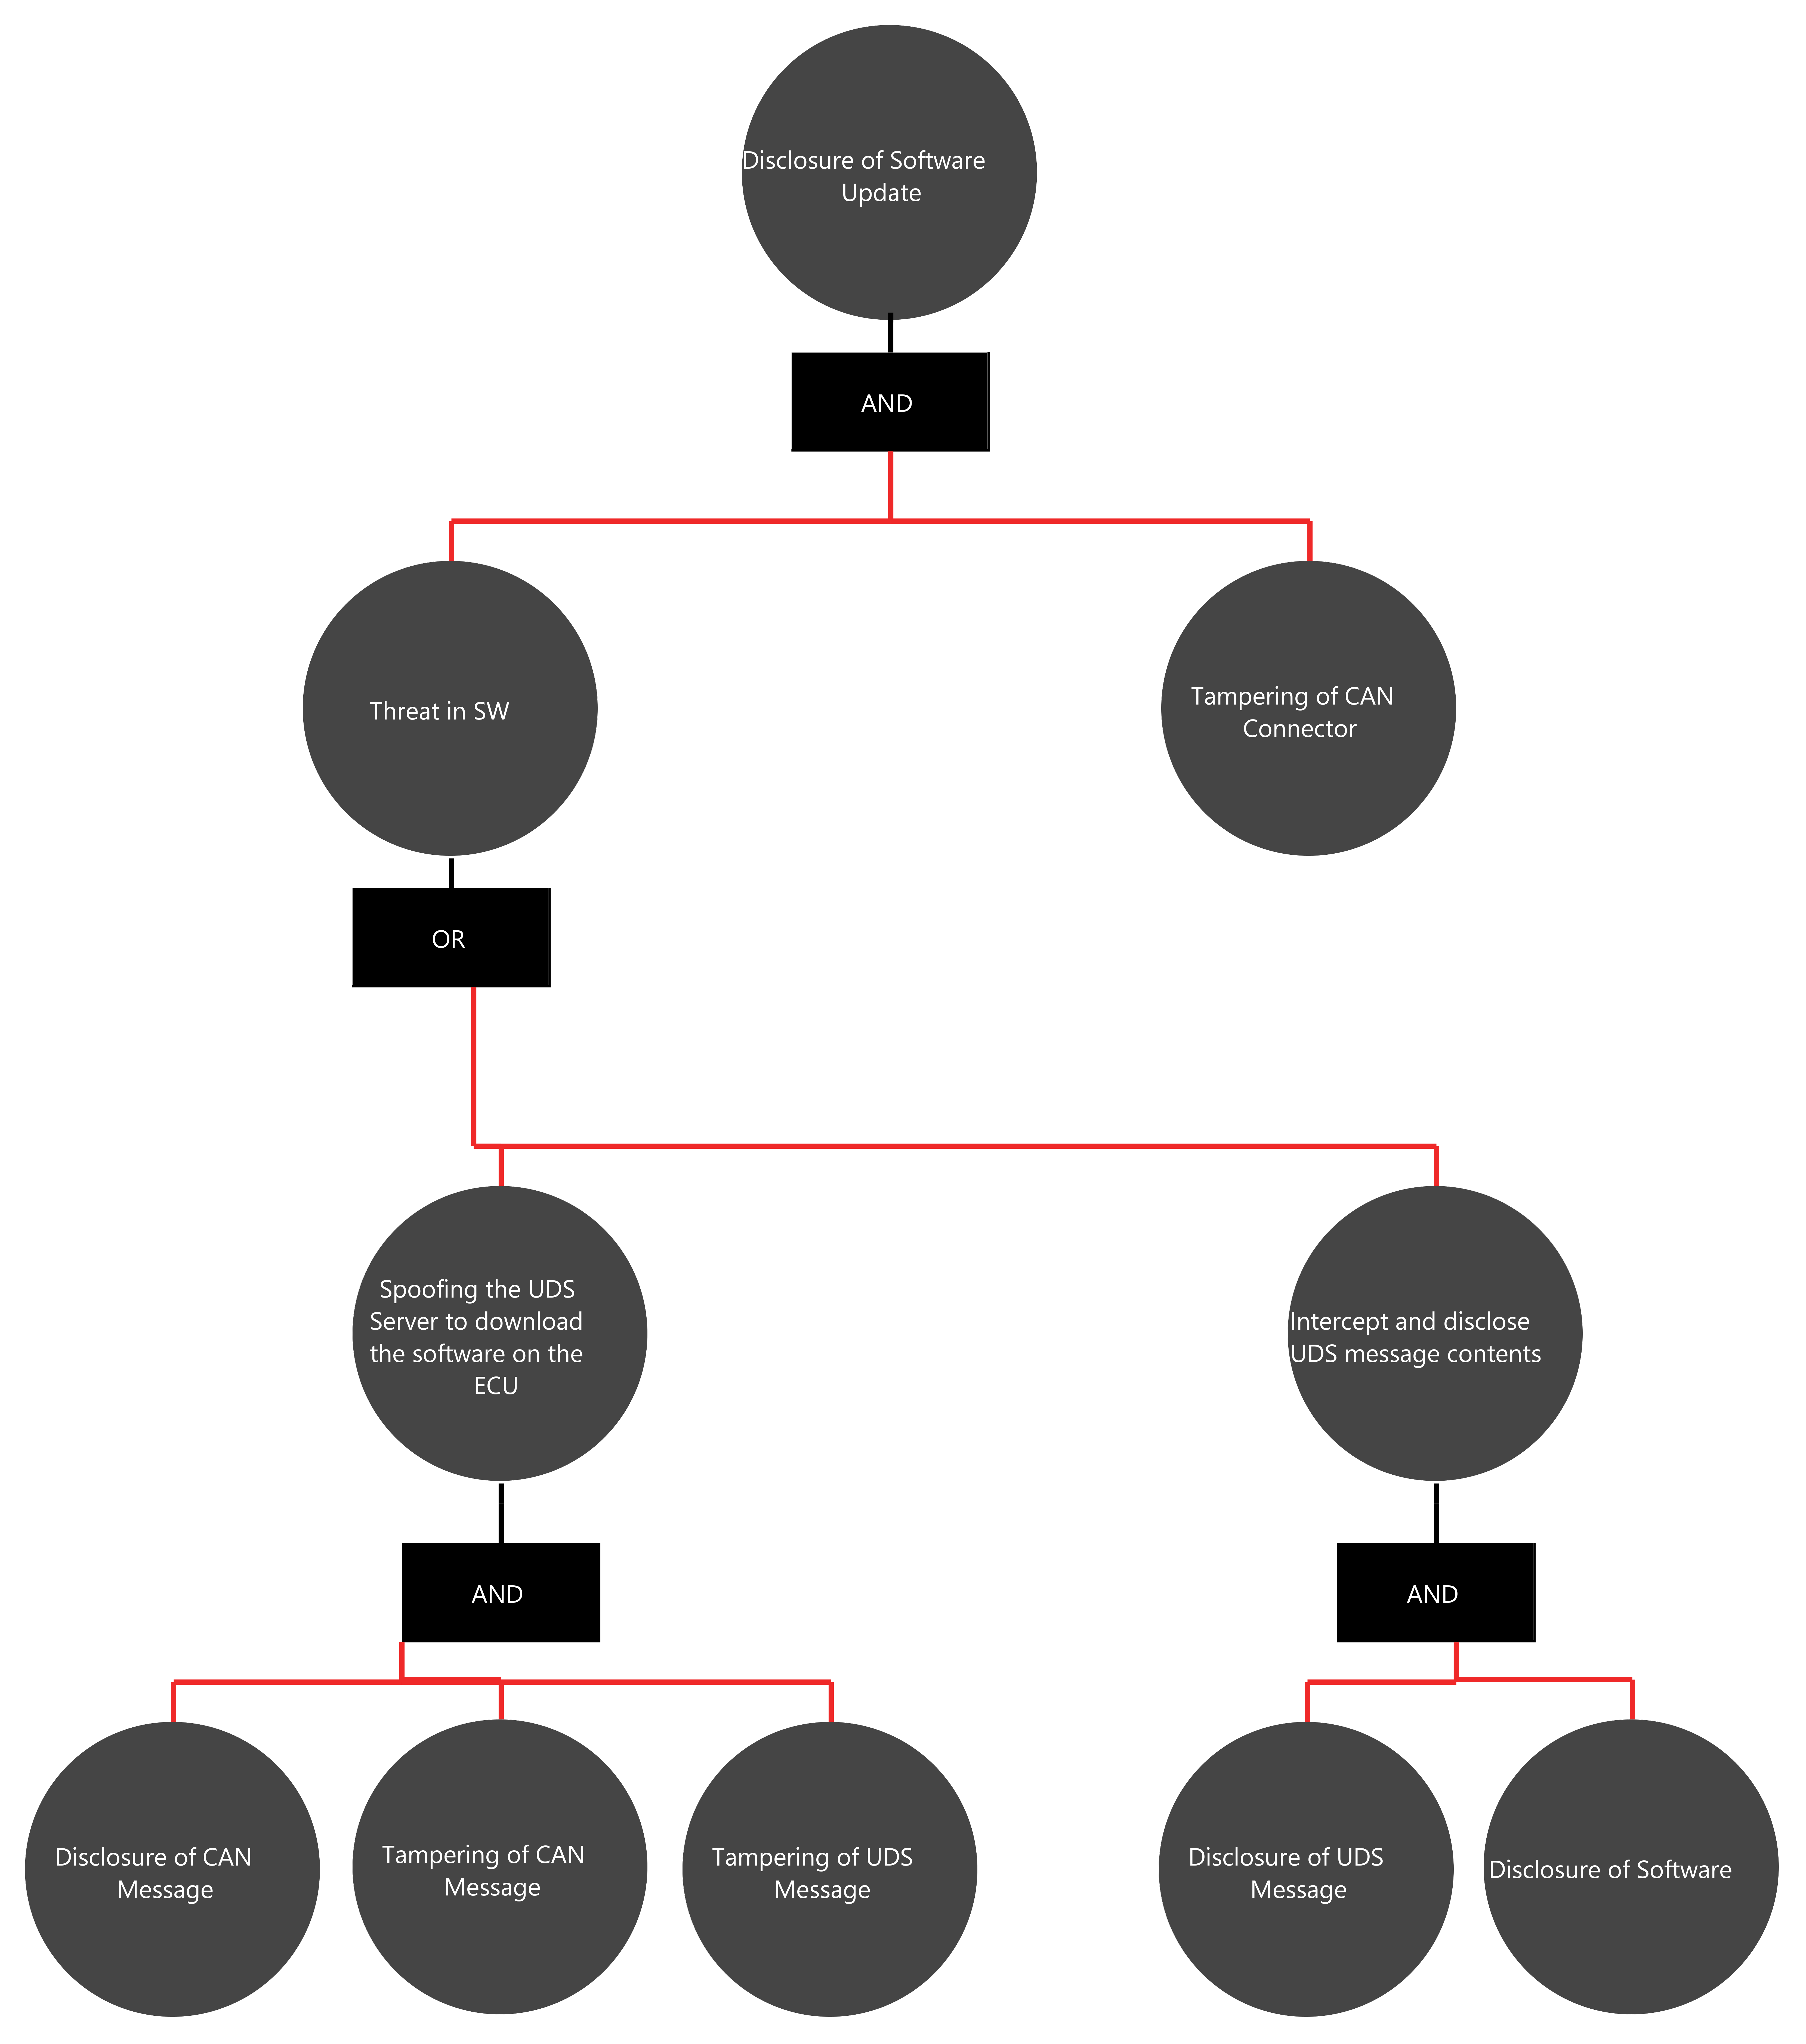
\includegraphics[width=120mm, keepaspectratio]{figures/AT-SECSW-00.png}
	\caption{Támadási fa a "Leak software" károkozáshoz} 
	\label{fig:ff_leak_sw}
\end{figure}

\newpage

A következő támadási fa a \textit{Change software} károkozáshoz készült és az \ref{fig:ff_change_sw} ábrán látható. 

Itt egyrészről különvettem egy \textit{Surveillance} pszeudo-fenyegetést, amely maga alá gyűjti azokat a fenyegetéseket amelyek önmagukban nem képesek a károkozást okozni, azonban ezt is kénytelenek előzetesen megtenni. A feltételezés az az, hogy a támadónak egy szoftver frissítési folyamatot le kell hallgatnia ahhoz, hogy a sajátját is véghez vigye. Itt egyrészről arról van szó, hogy a támadó azonosítja az ECU-kat a CAN és UDS üzenetek metaadatai alapján, valamint a szoftver felépítését is szükséges azonosítania ahhoz, hogy végül egy saját szoftvert is képes legyen az eszközre feltölteni.

Emellett egyértelműen szükséges a HW oldaláról a CAN busz integritásának megváltoztatása, hogy a támadó képes legyen a saját üzeneteit elküldeni a célpont ECU-nak.

Végül maga a szerkesztett vagy saját szoftver feltöltés lesz a következő lépés, ez magával vonja mind az egyedi CAN és UDS üzenet illetve szoftver létrehozását a támadó oldalról, úgy, hogy azt a célpont ECU elfogadja.

Megfigyelhető, hogy itt egyébként nincs szükség erre a szegmentálásra, hiszen minden atomi fenyegetésnek jelen kell lennie a rendszerben a rendszerszintű fenyegetés aktiválásához, viszont ebben a formában átláthatóbb és funkcionálisan nincs hatással az elemző eszköz működésére ez a formátum.

\begin{figure}[!ht]
	\centering
	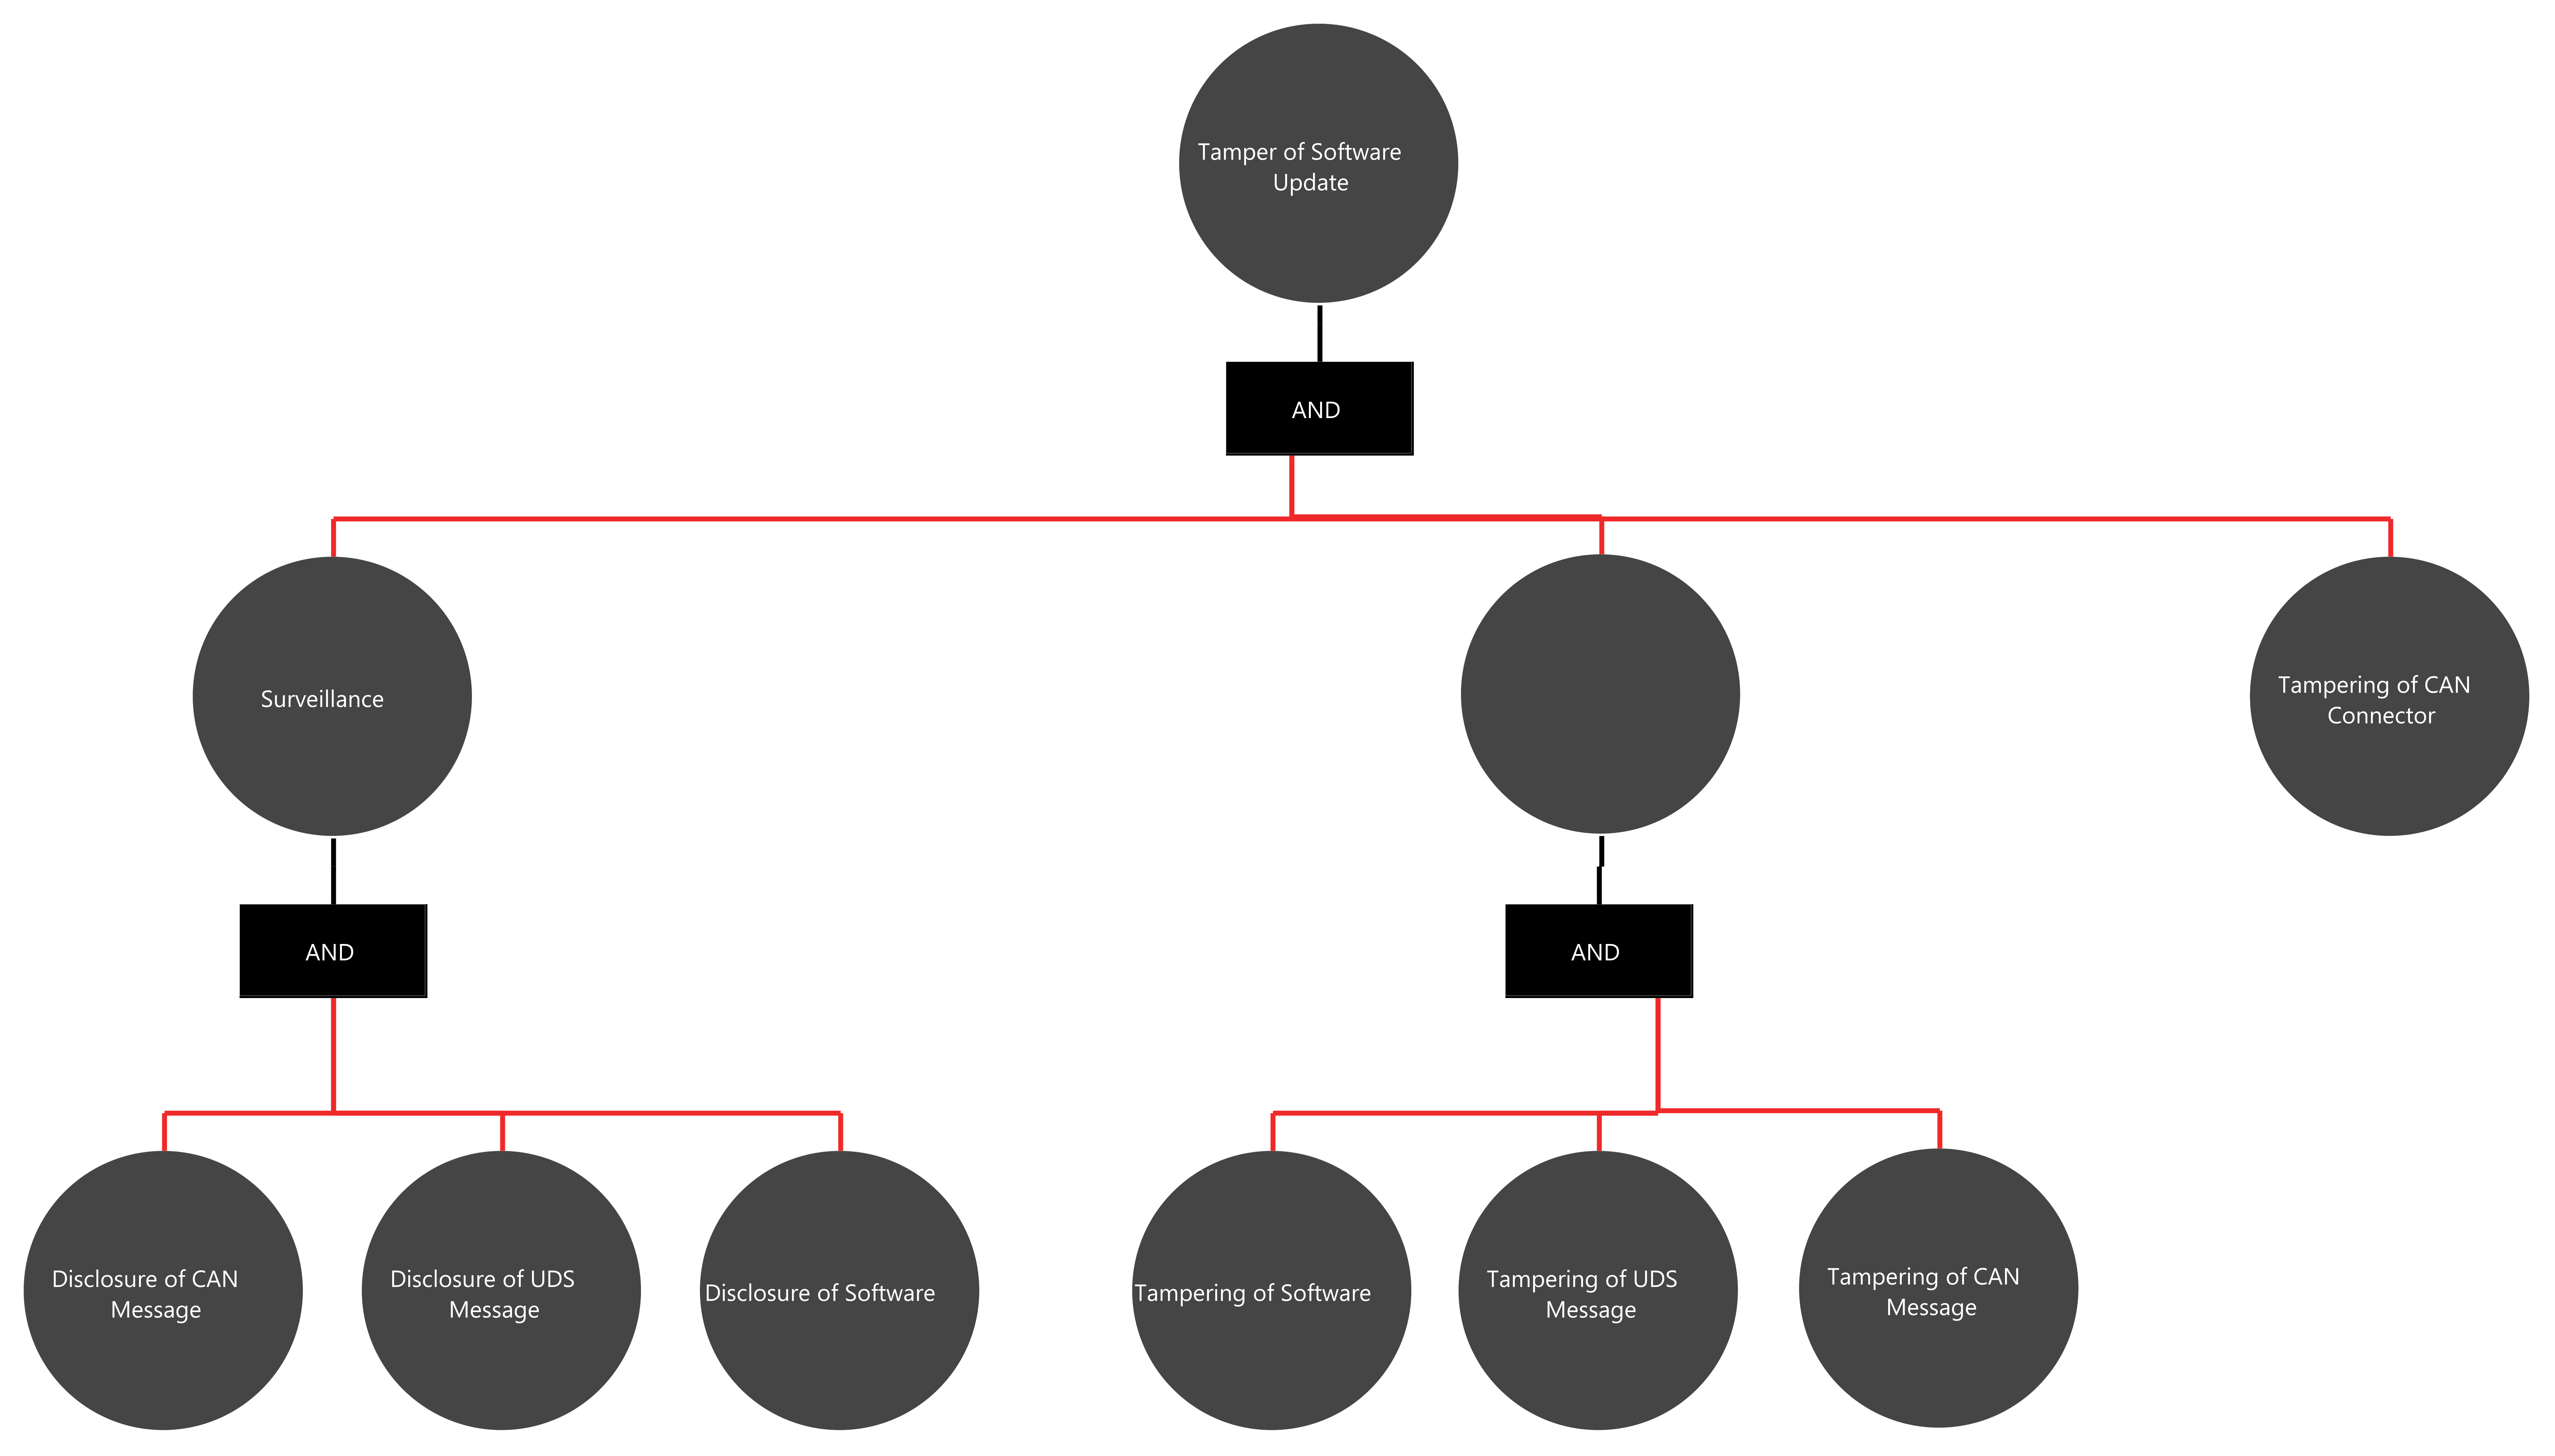
\includegraphics[width=120mm, keepaspectratio]{figures/AT-SECSW-01.png}
	\caption{Támadási fa a "Change software" károkozáshoz} 
	\label{fig:ff_change_sw}
\end{figure}

\newpage

A szoftver elérhetőségének módosítására az \ref{fig:ff_remove_sw} ábrán láthatjuk a támadási fát. Ez a támadás már sokkal több módon elvégezhető, a kár kisebb a többi esethez képest azonban az elvégzéséhez szükséges tudás is a támadó részéről.

Egyrészről az első szinten külön vettem a HW-es kapcsolat megszüntetését amely egy fizikai hozzáférést jelentene a járműhöz attól ami potenciálisan távolról is elvégezhető.

A távolról elvégezhető esetben lehetőség szerint a támadó egyrészről sértenie kell a CAN busz integritását másrészről vagy az érkező üzenetek blokkolását kell elérnie, ezzel a szoftver funkcionalitását blokkolva vagy azokat úgy módosítva, hogy utána a célpont ECU ne fogadja el azokat (pl. szálított adat módosítása úgy hogy a CRC nincs módosítva egyenesen vezetne az üzenet eldobásához üzembiztonsági elvárások miatt).

\begin{figure}[!ht]
	\centering
	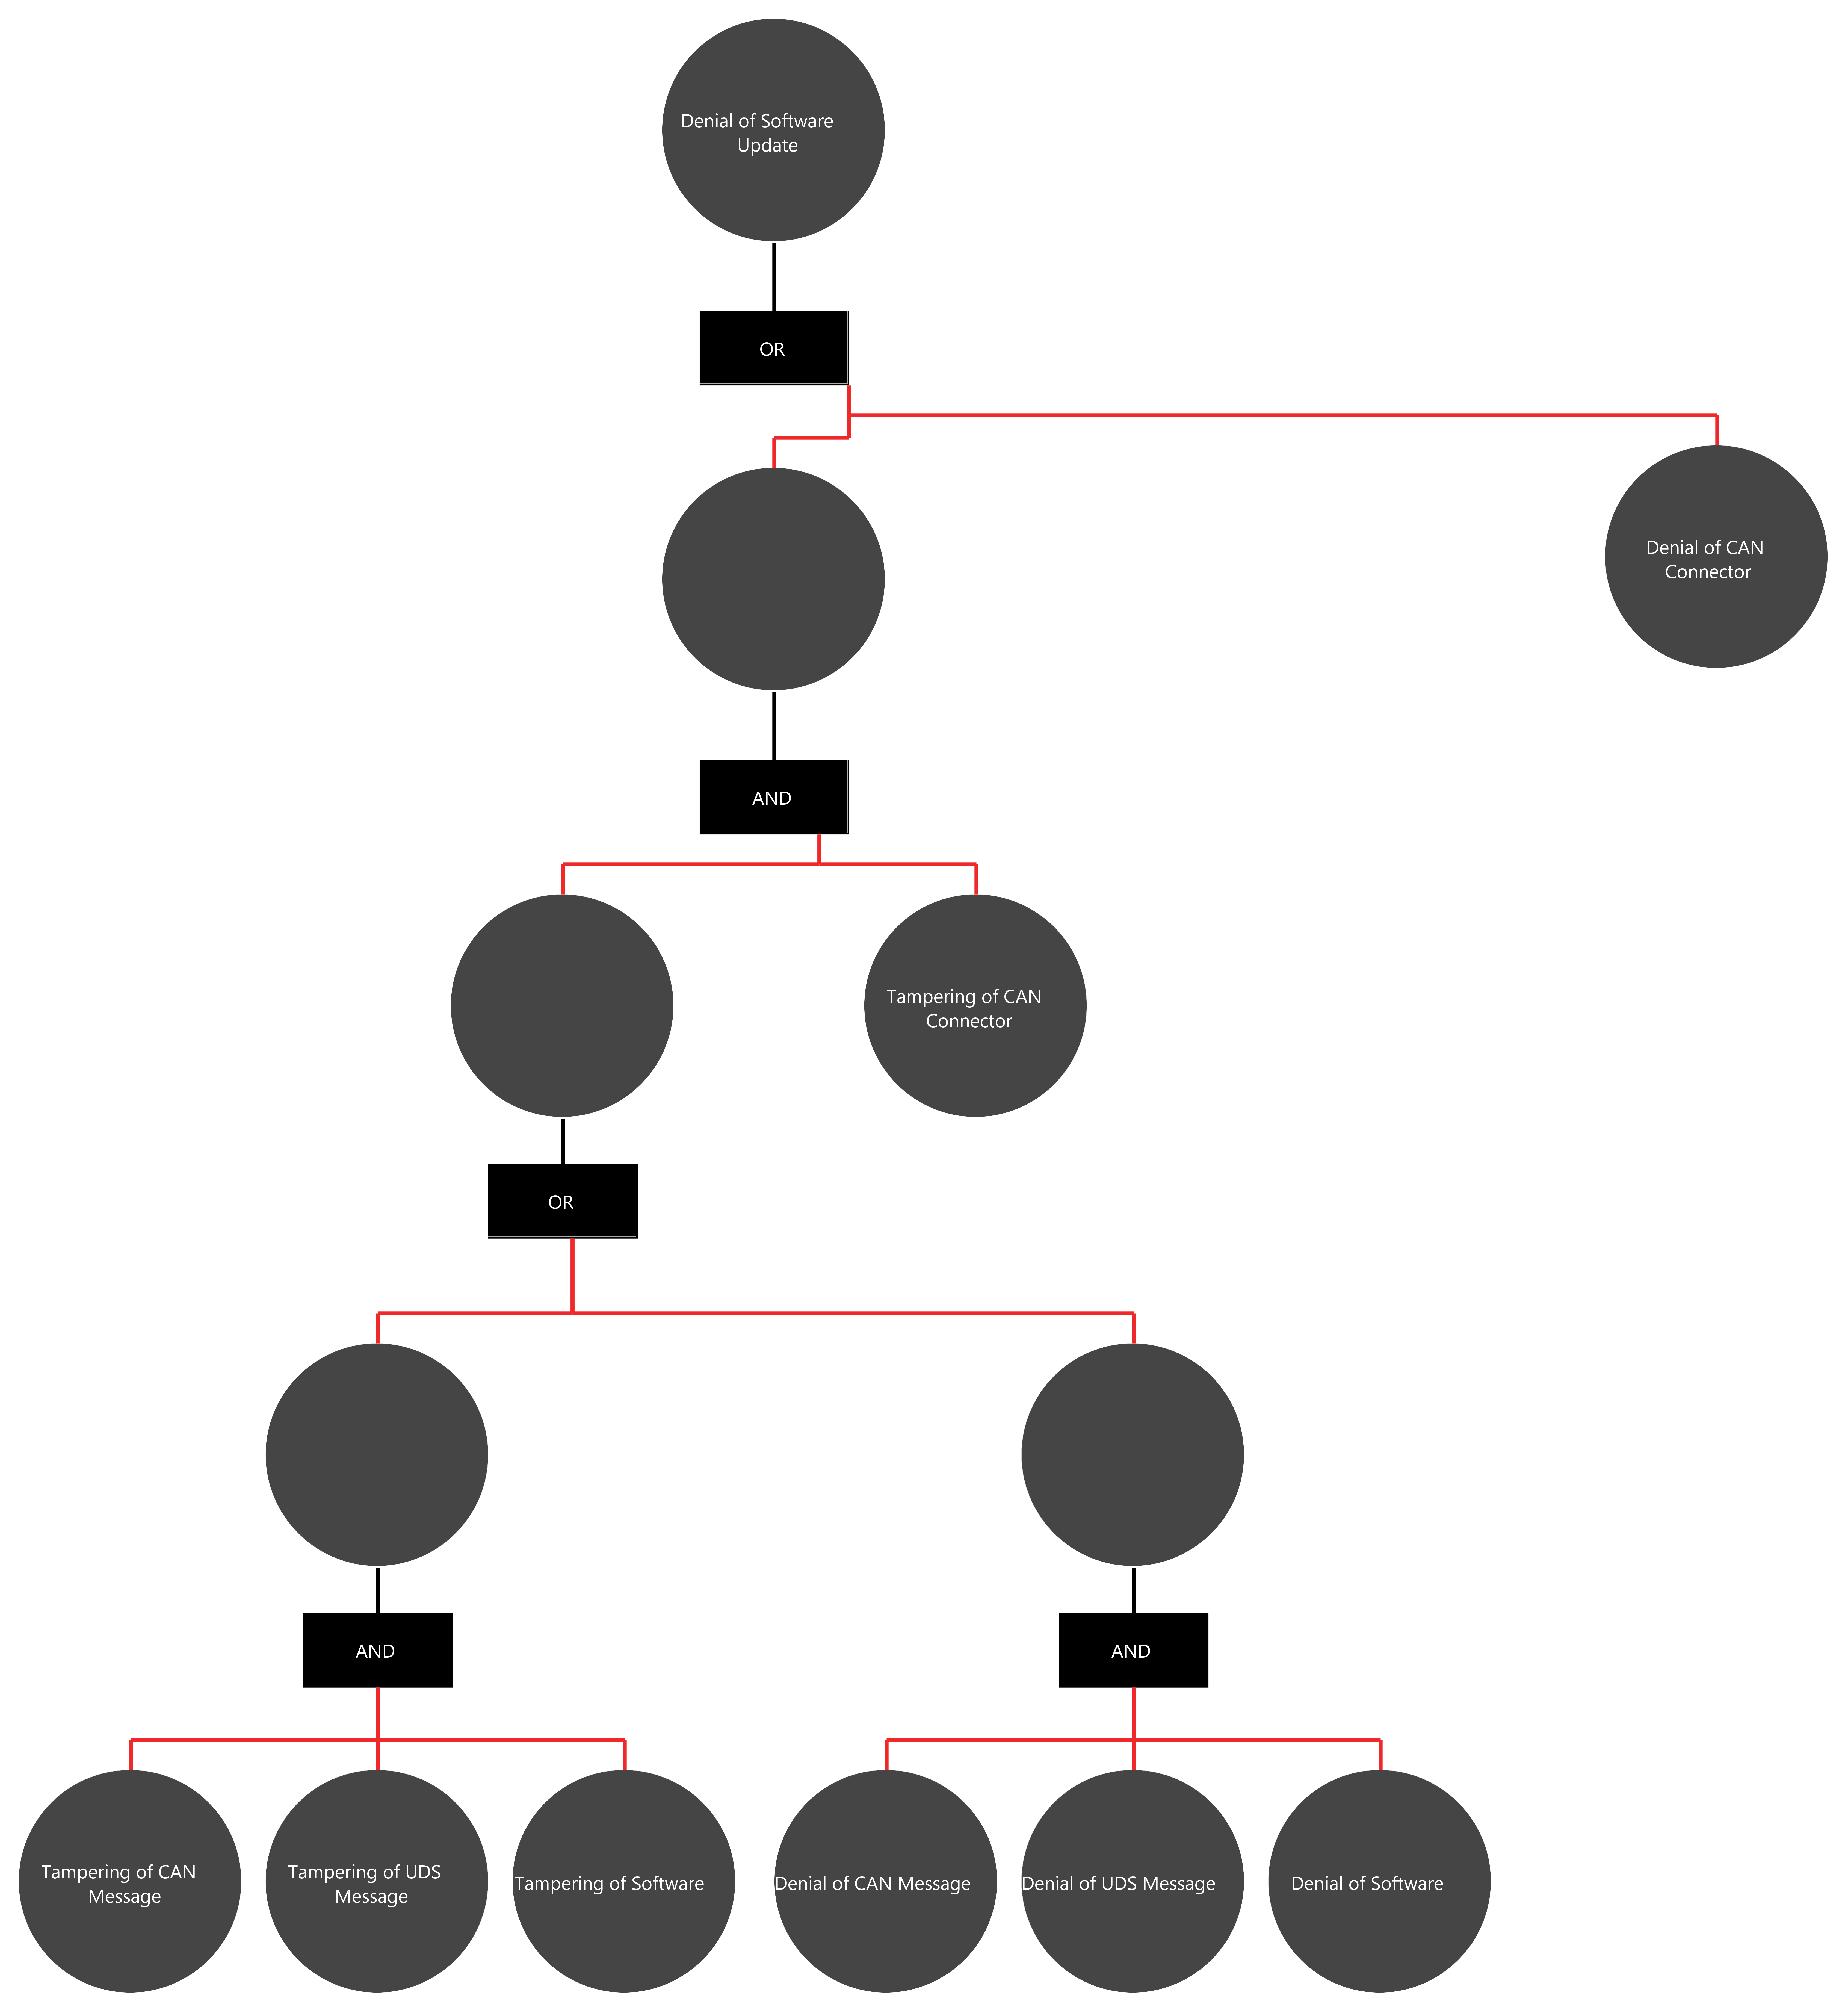
\includegraphics[width=120mm, keepaspectratio]{figures/AT-SECSW-02.png}
	\caption{Támadási fa a "Remove software" károkozáshoz} 
	\label{fig:ff_remove_sw}
\end{figure}

\newpage

Áttérve a diagnosztikai adatok szivárogtatására az \ref{fig:ff_leak_data} ábrán, itt is alapvetésnek vesszük a CAN busz integritásának változását valamint magát az adatszivárgást.

A következő szinten két utat különböztetünk meg az információkhoz való hozzáférésnél, egyik esetben a bejövő üzenetek lehallgatása és visszafejtése lehet a támadó megoldása. A másik bonyolultabb esetben olyan üzeneteket kell a támadónak konstruálnia amelyeket a célpont ECU tud értelmezni valamint, megfelelőnek és jogosultnak ítél.

\begin{figure}[!ht]
	\centering
	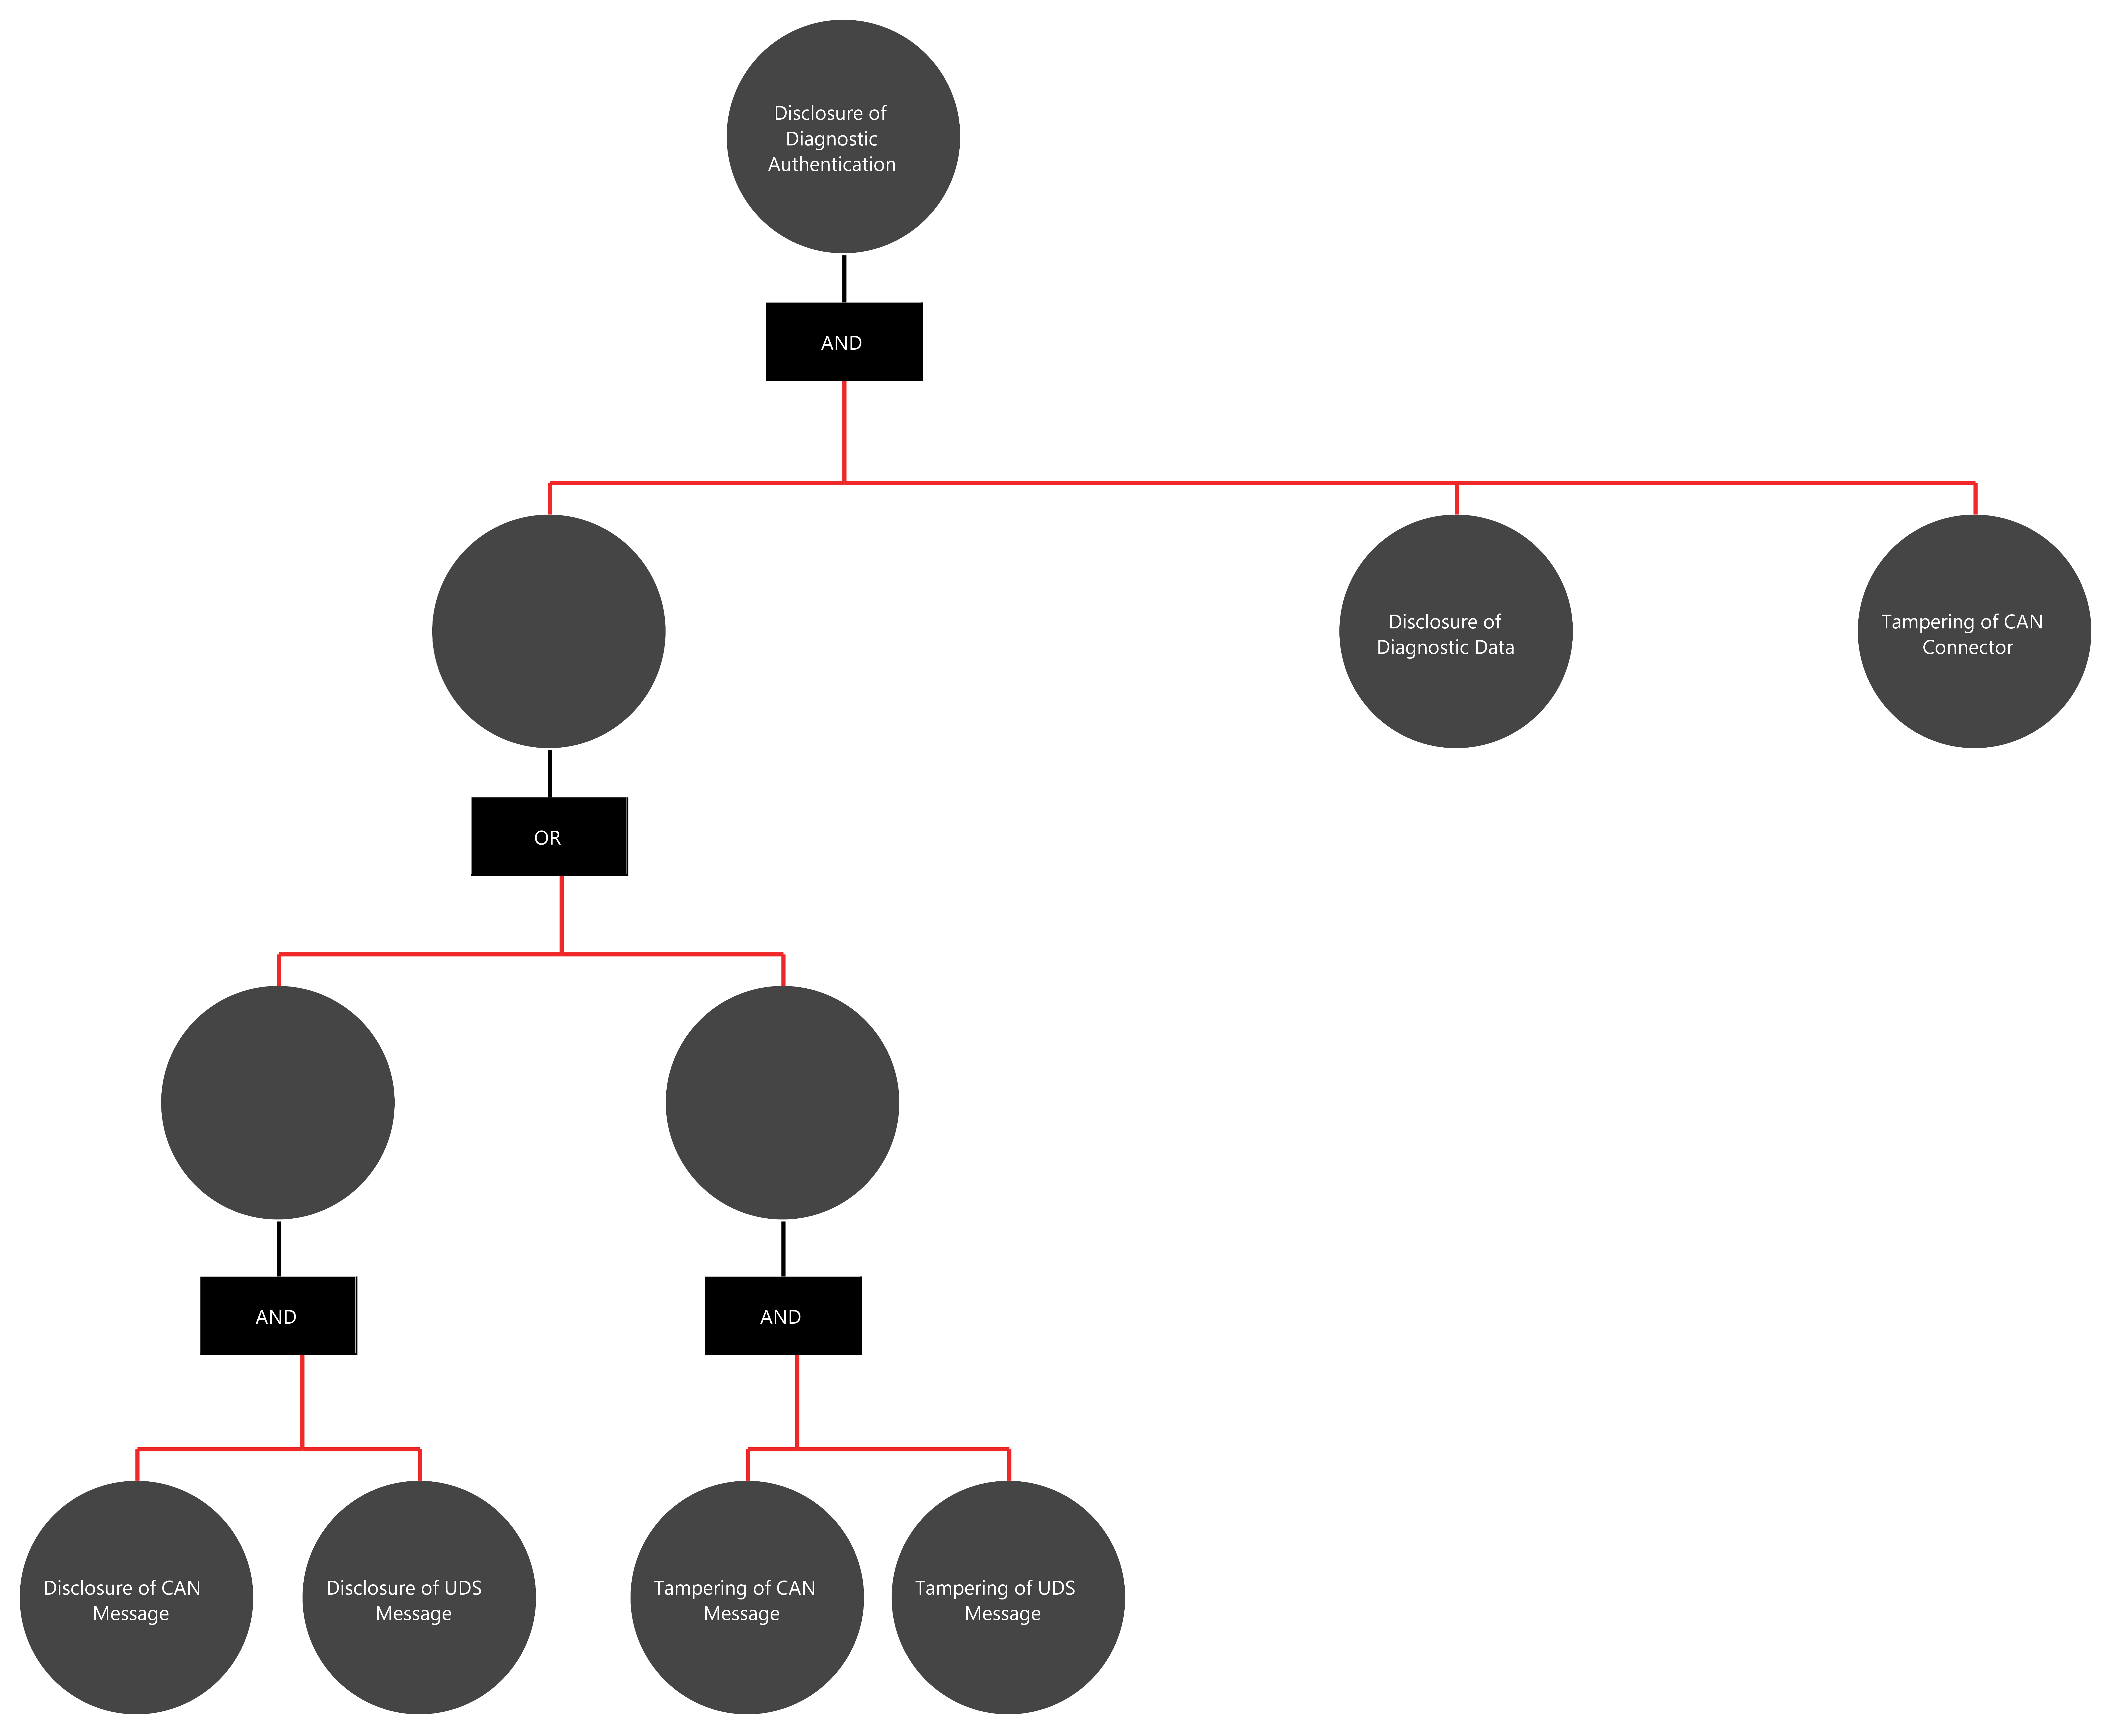
\includegraphics[width=120mm, keepaspectratio]{figures/AT-SECDIAG-00.png}
	\caption{Támadási fa a "Leak confidential data" károkozáshoz} 
	\label{fig:ff_leak_data}
\end{figure}

\newpage

Az \ref{fig:ff_access} ábrán, azt a támadási fát keressük amelyikkel a támadó hozzáférhet korlátozott elérésű diagnosztikai szolgáltatásokhoz. Hasonlóan a szoftver megváltoztatásához itt is szükségeltetik egy lehallgatási lépés, valamint ezen túl a megfelelő üzenetek konstruálása amely különböző mitigációk segítségével jól védhető.

\begin{figure}[!ht]
	\centering
	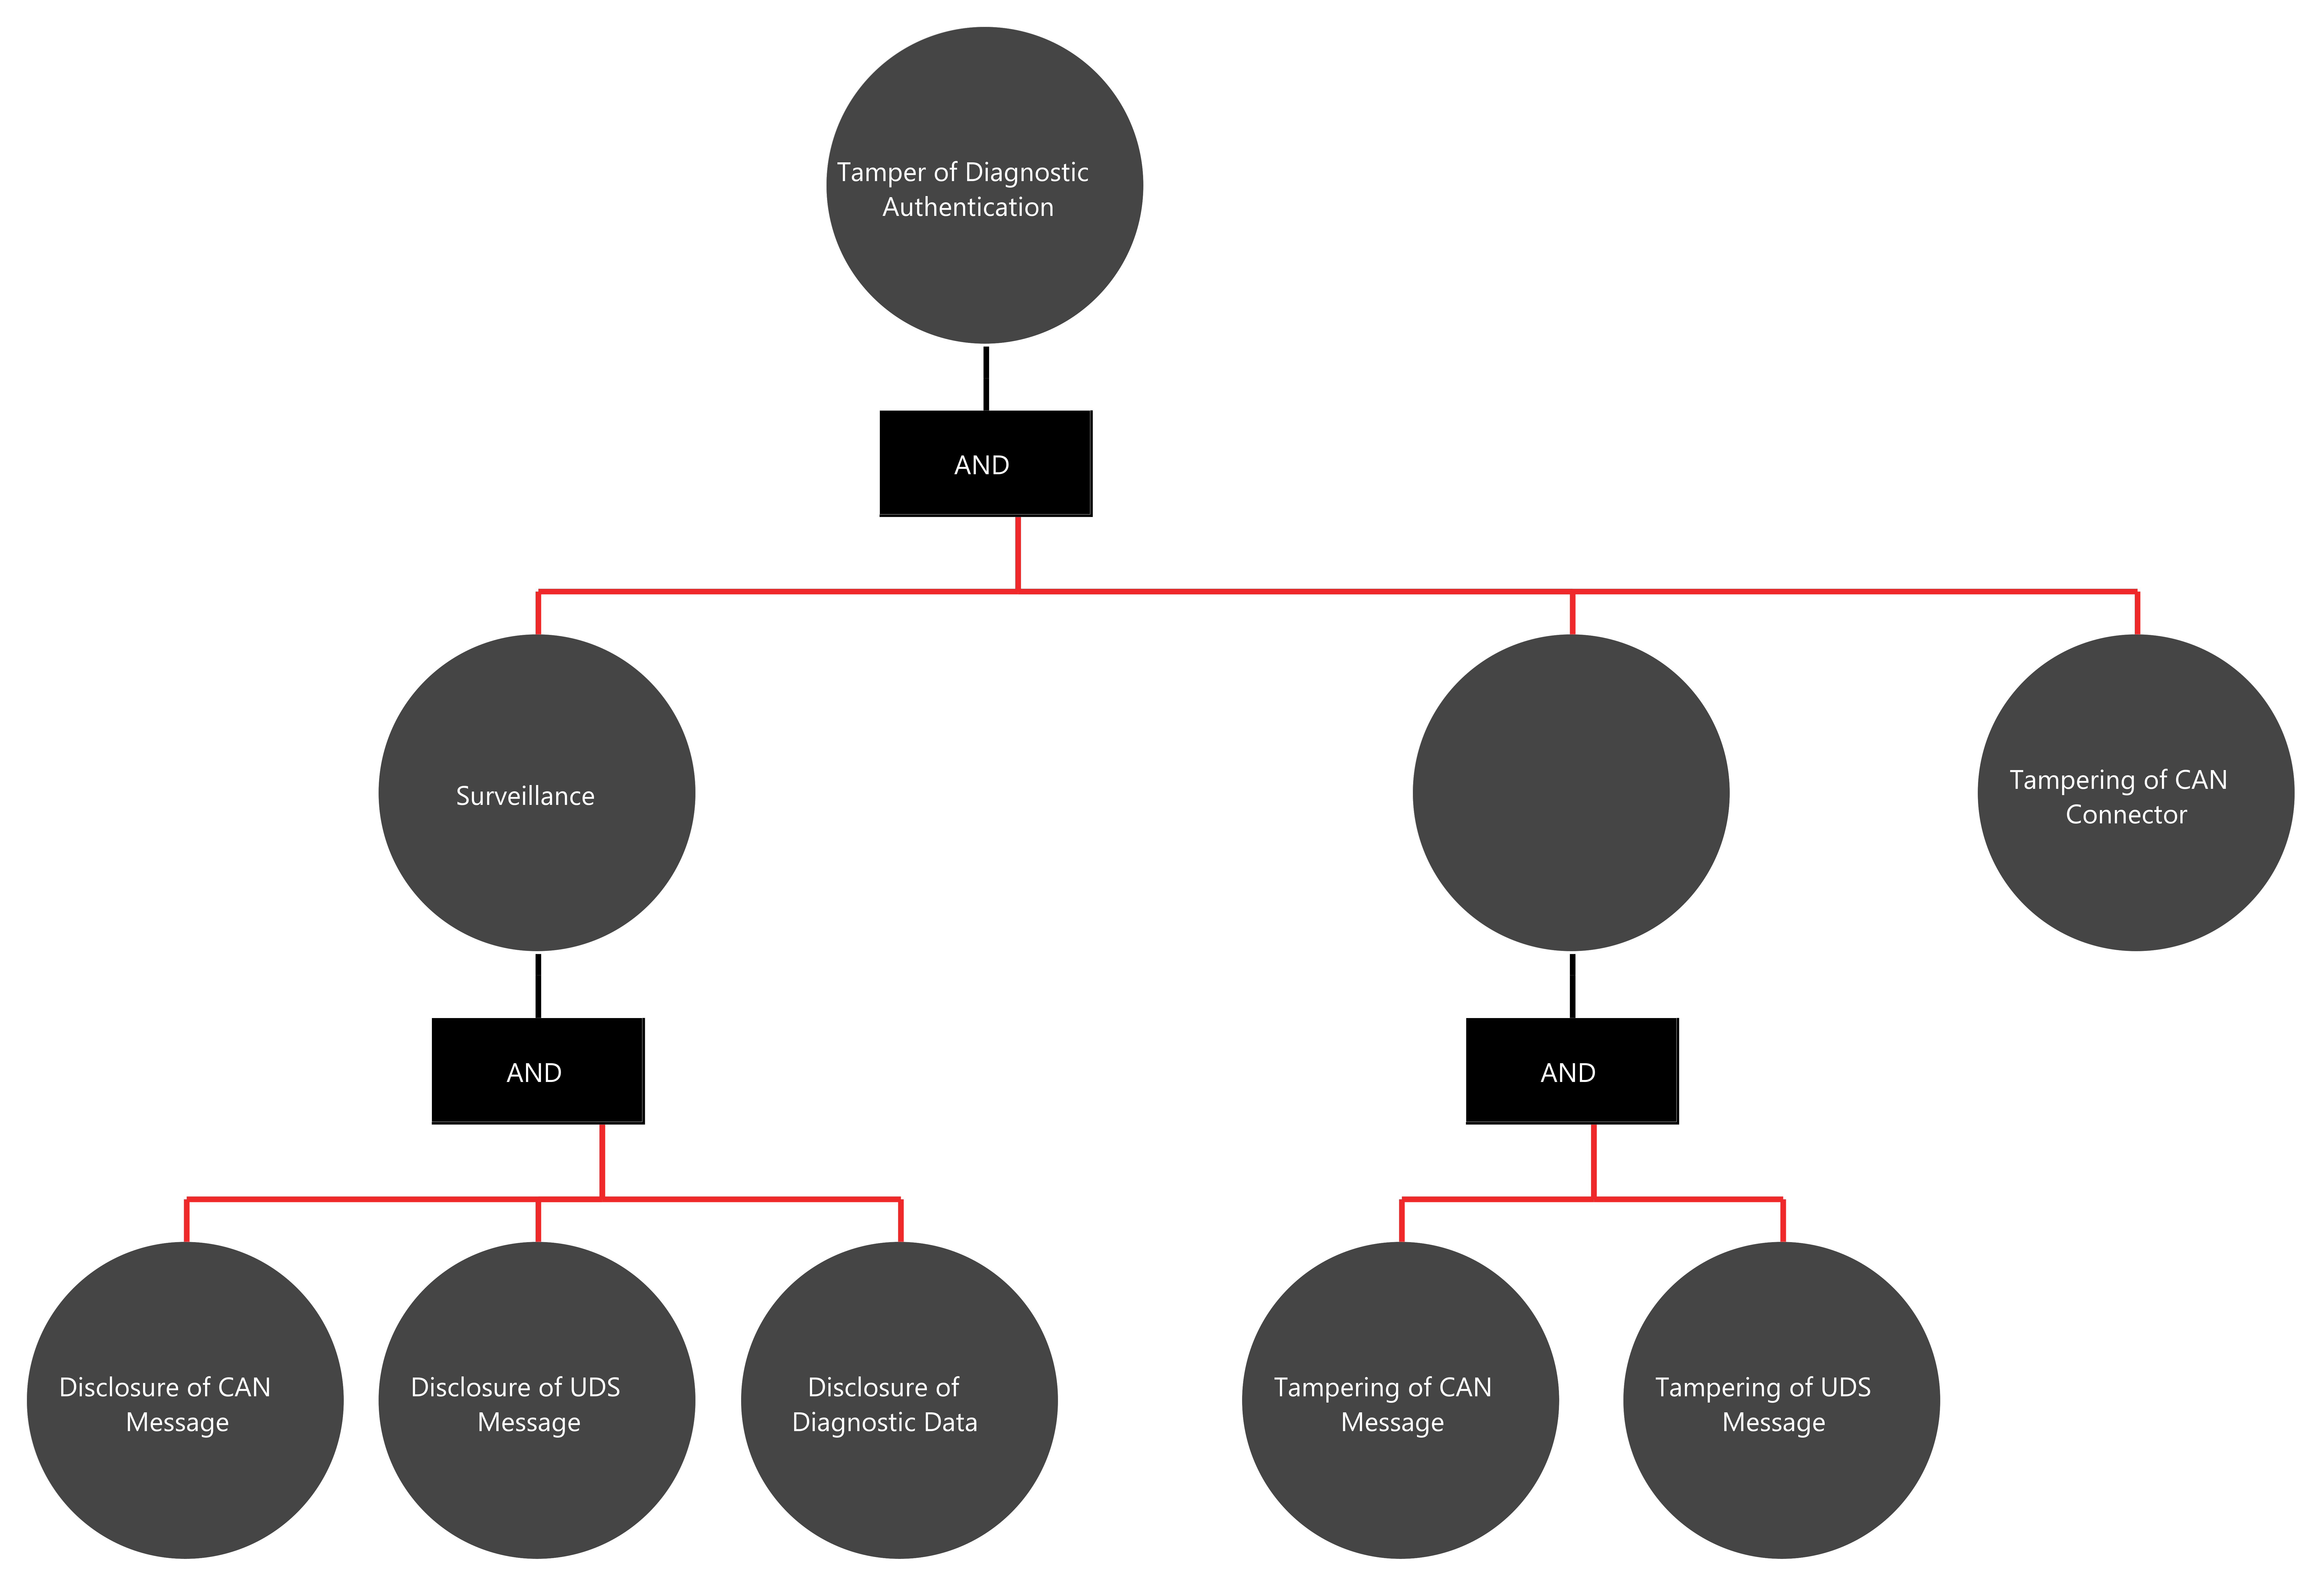
\includegraphics[width=120mm, keepaspectratio]{figures/AT-SECDIAG-01.png}
	\caption{Támadási fa a "Access unauthorized functionality" károkozáshoz} 
	\label{fig:ff_access}
\end{figure}

\newpage

Az \ref{fig:ff_block_auth} ábrán, az autentikációs lépések blokkolását okozó támadási fa látható. Ez is megegyezik a szoftver frissítés elérhetőségét sértő fához. Ennek az oka ezúttal is az, hogy a műveletet mivel mindkettő diagnosztikai szolgáltatás, ugyanazon lépésekkel kell megtenni ezen az absztrakciós szinten.

\begin{figure}[!ht]
	\centering
	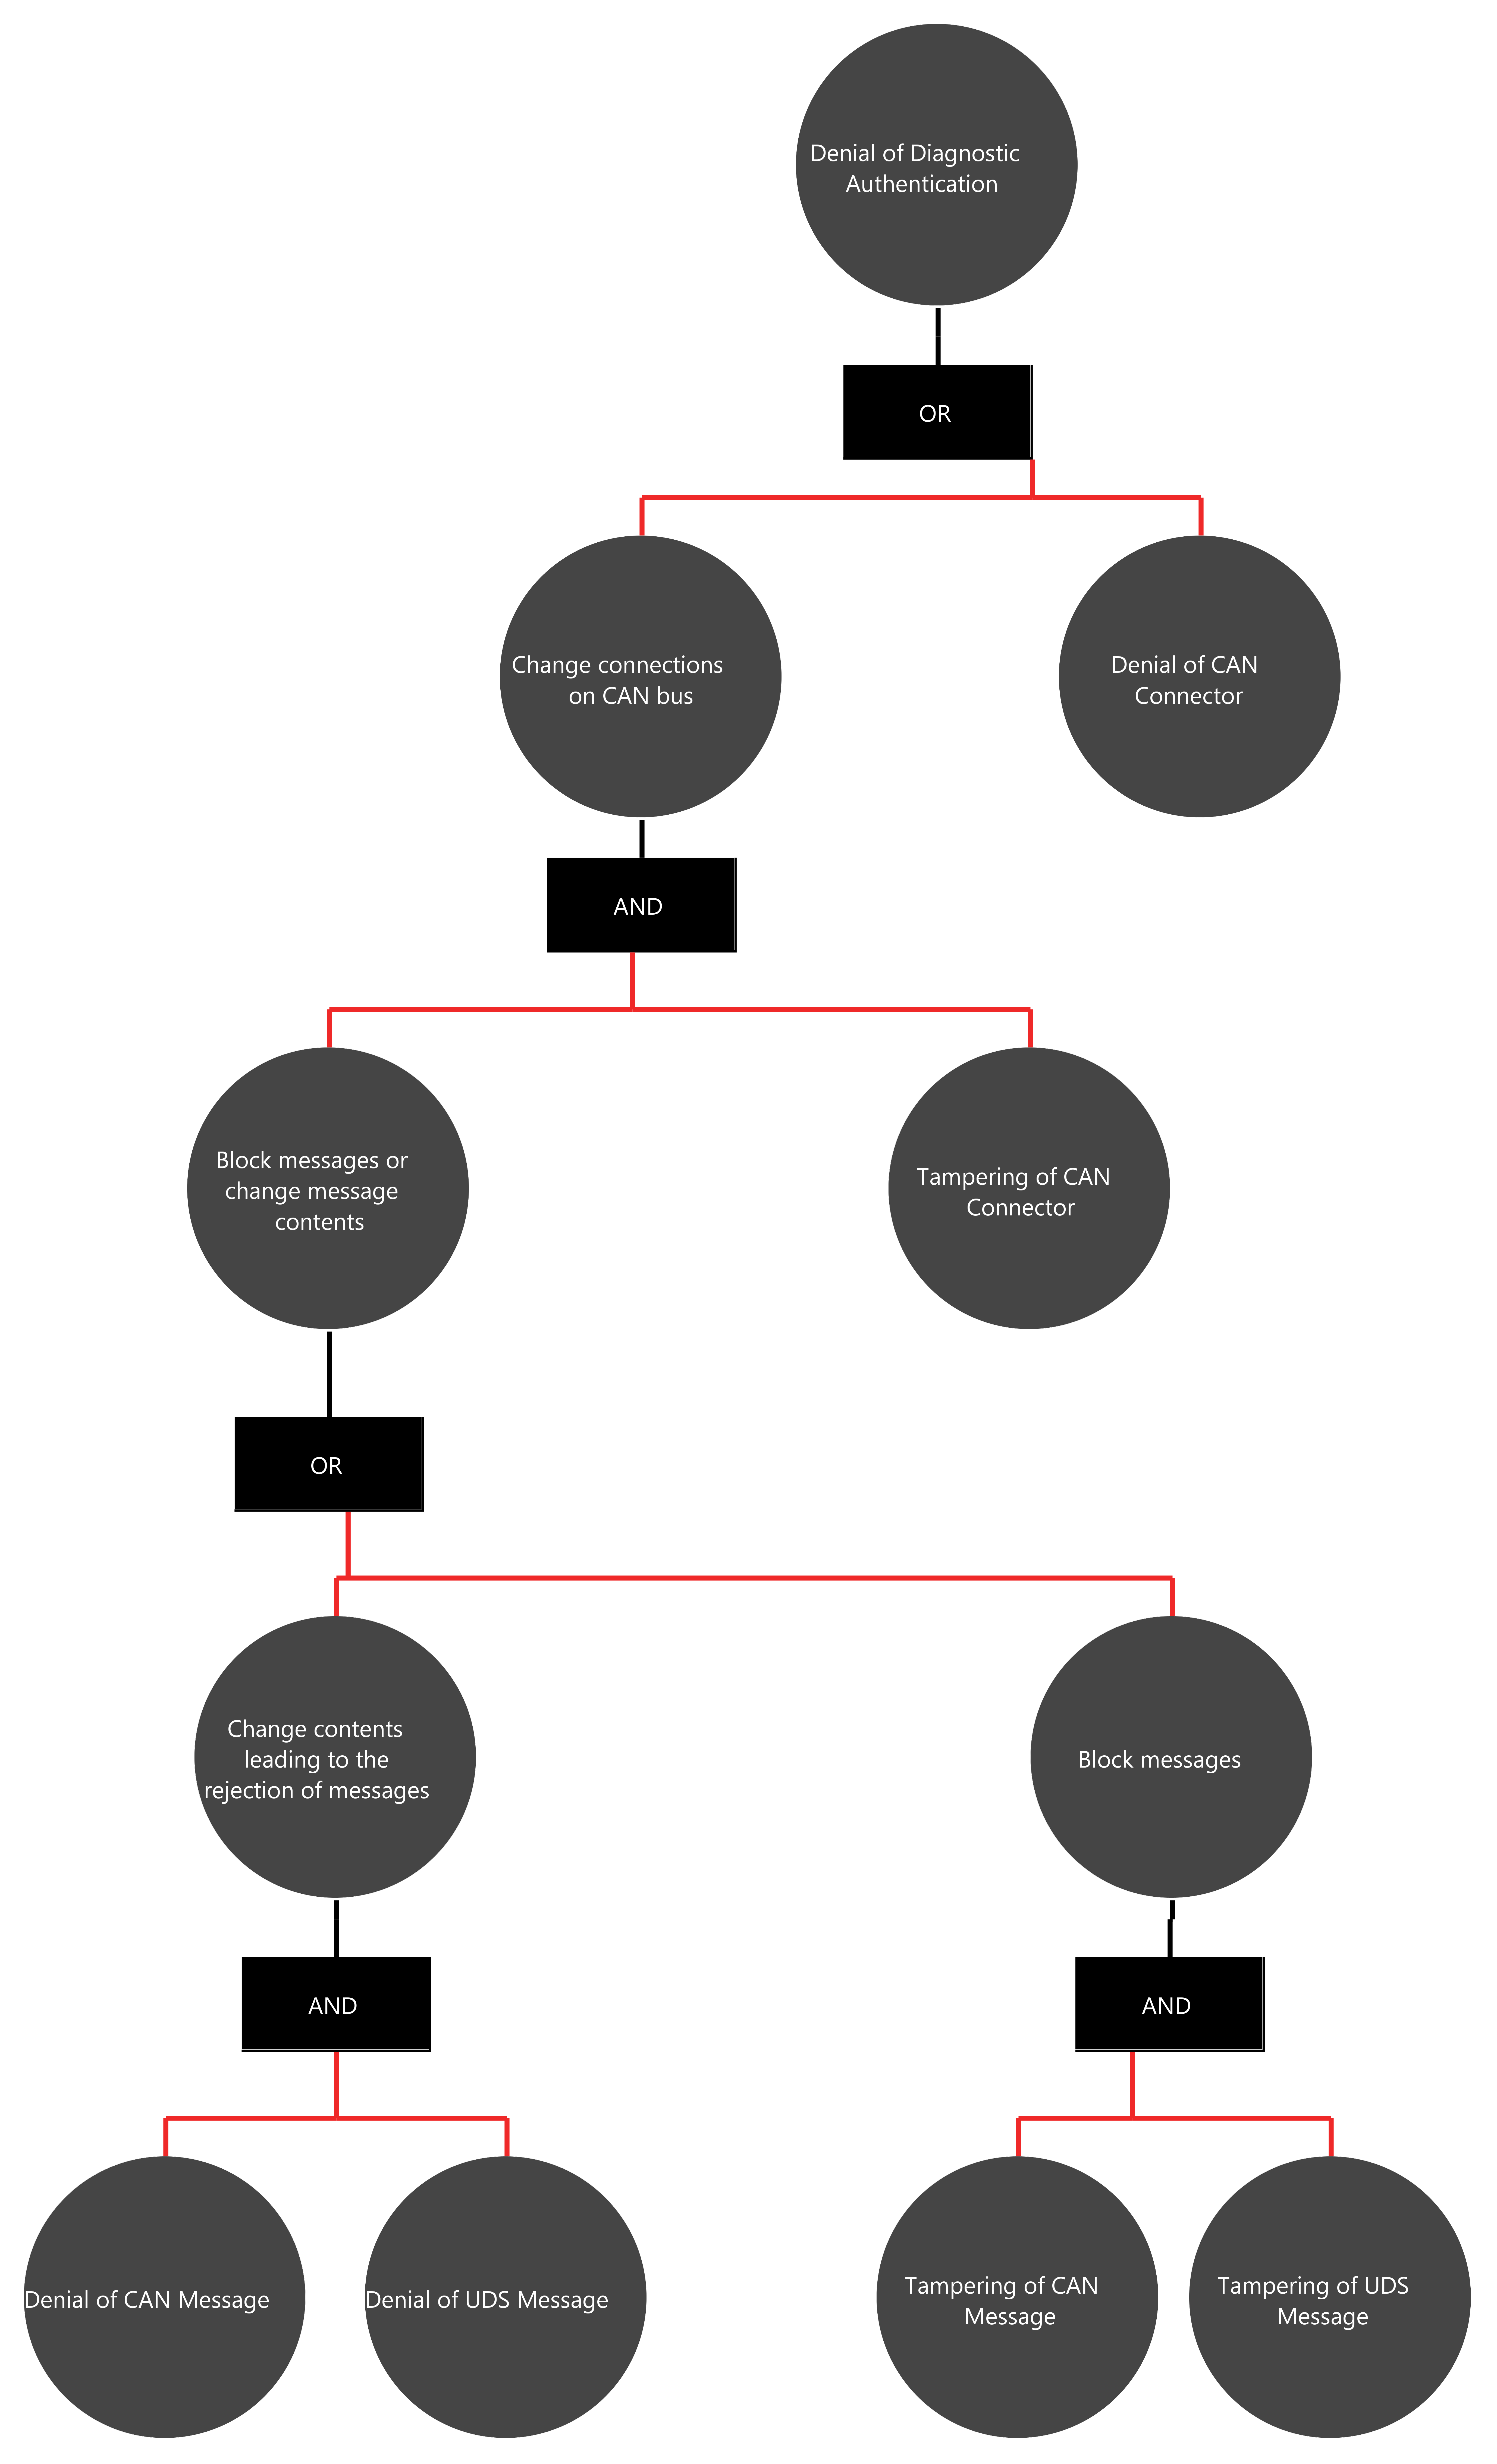
\includegraphics[width=120mm, keepaspectratio]{figures/AT-SECDIAG-02.png}
	\caption{Támadási fa a "Block authentication attempts" károkozáshoz} 
	\label{fig:ff_block_auth}
\end{figure}

Összességében elmondható, hogy a támadási fák konstruálása helyes, ezt bizonyítja az is, hogy a diagnosztikai rutinok támadási fái ugyanazon mintákat követik hiszen ugyan azon értékeket használja a két szolgáltatás. Amennyiben a szoftvert és a diagnosztikai adatot egy absztraktabb \textit{adat} meghatározással jelöltük volna a termékleírásban úgy elég lett volna kevesebb támadási fa azonban, ezeknek a külön vétele a manuális analízishez szükséges.

Szintén elmondható, hogy az eljárás gyors és ezáltal könnyen megismételhető. Ezen támadási fáknak a konstruálása ugyanazon atomi és legfelső eseményekből áll így a kontextus váltás a külön fák konstruálásakor jóval egyszerűbb.

Végül pedig a teljességet is teljesíti a támadási fa, minden termékleírásban valamint fenyegetésmodellben meghatározott érték elleni fenyegetés szerepel valamely támadási fában egyrészről, másrészről pedig megteremtettünk egy lekövethetőséget (traceability) a SW-, illetve HW-szintű fenyegetések valamint a károkozások között.

\section{Manuális analízis}

Az utolsó lépése az elemzésnek a manuális analízis. Itt először a hatásérték elemzést, utána pedig a támadás megvalósíthatóság elemzést végezzük el.\\

Ahogy az a \ref{fig:ff_imprate} ábrán látható a SFOP értékek mentén meg lettek határozva a hatásértékei az egyes károkozásoknak.

A legkomolyabb hatások a szoftver megváltoztatásával, törlésével, valamint a korlátozott hozzáférésű funkcionalitások használata lettek. Ezek értelemszerűen nagyobb kockázatot is jelentenek mint mondjuk az autentikációnak a blokkolása. Az elemzés az ISO 21434 \cite{ISO21434} által ajánlott és annak a függelékében lévő példa elemzések mintájára készültek el.\\

\begin{figure}[!ht]
	\centering
	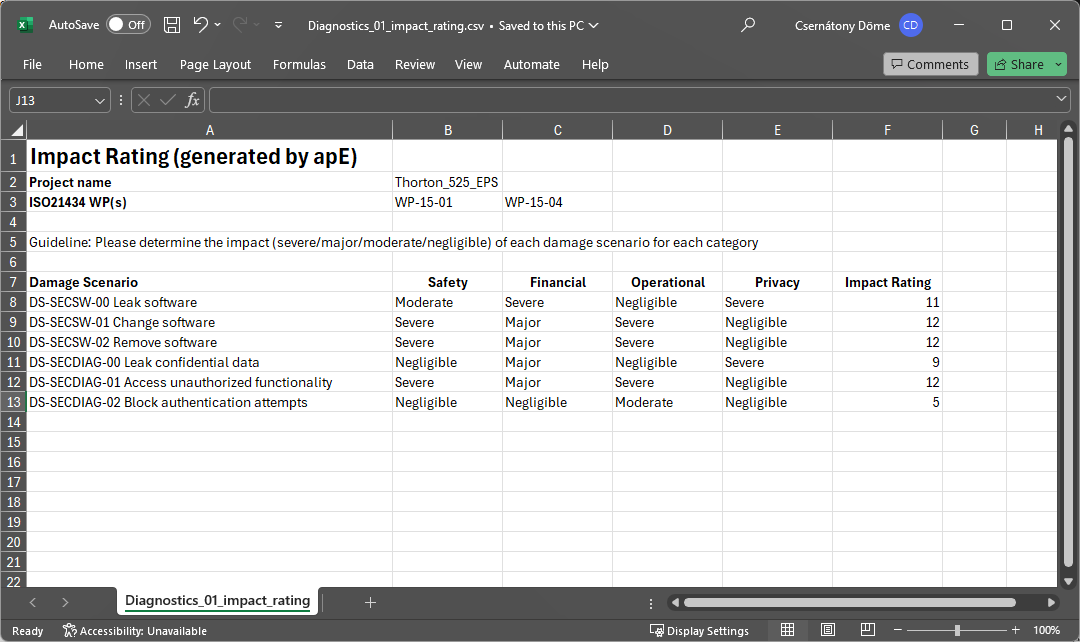
\includegraphics[width=120mm, keepaspectratio]{figures/ff_imprate.png}
	\caption{Hatásérték elemzés} 
	\label{fig:ff_imprate}
\end{figure}

Az \ref{fig:ff_attfeas} ábrán látható az értékelés az Attack Potential Based megközelítést használja, ez szintén az egyik ajánlása az ISO 21434 \cite{ISO21434} szabványnak, valamint szintén annak a függelékében lévő minta alapján készült el ez az elemzés is.

Ezen kiértékelések történhetnek egy szakértő által egyénileg, több stakeholder bevonásával illetve behatolástesztelő mérnökök támogatásával. A kiértékelés a támadó képességei és a rendelkezésre álló információk alapján ad egy becslést a támadási utak megvalósíthatóságára.

\begin{figure}[!ht]
	\centering
	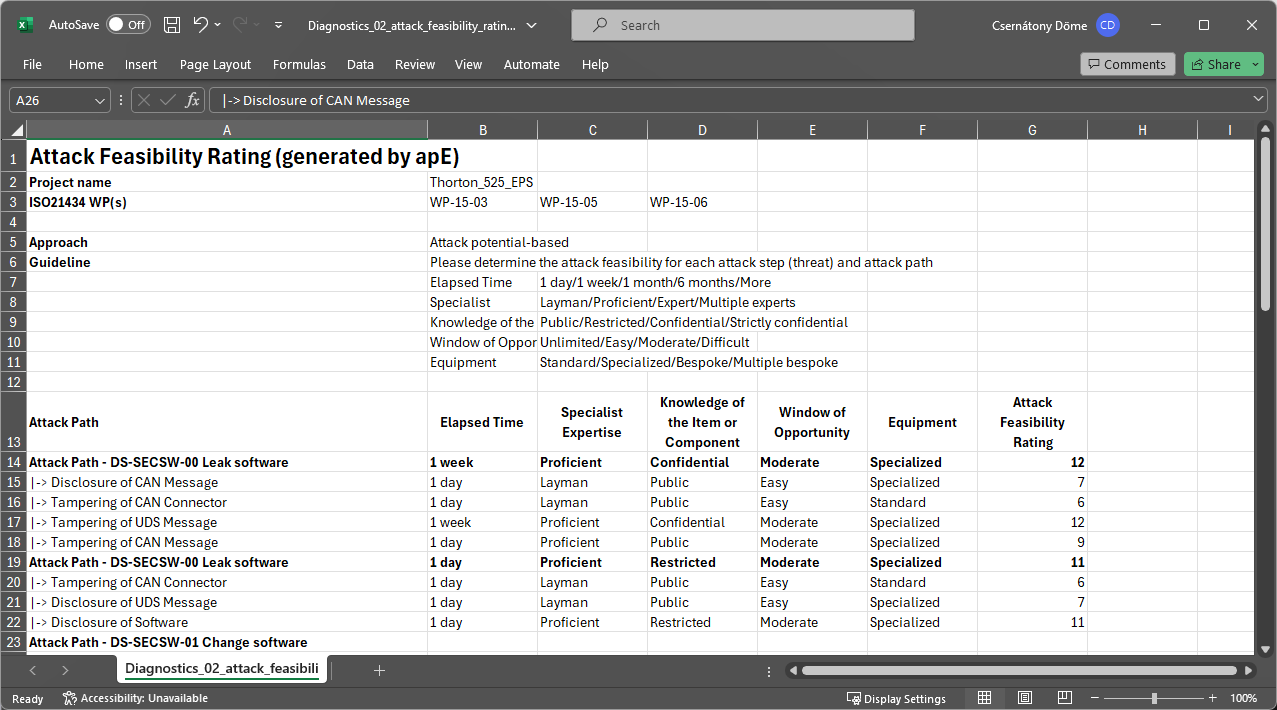
\includegraphics[width=120mm, keepaspectratio]{figures/ff_attfeas.png}
	\caption{Támadás megvalósíthatóság elemzés a "Leak software" károkozáshoz} 
	\label{fig:ff_attfeas}
\end{figure}

Ezzel befejezve a manuális analízisek eredményeinek a szabvány által leírt kombinációja alapján fog a kiberbiztonsági mérnök előállni a kockázati értékekkel amelyek mentén lehet eldönteni mely támadások azok amelyek valóban nagy kockázattal járnak és amelyekre védelmet kell biztosítani valamilyen formában.